%!TEX root = ../template.tex
%%%%%%%%%%%%%%%%%%%%%%%%%%%%%%%%%%%%%%%%%%%%%%%%%%%%%%%%%%%%%%%%%%%%
%% chapter2.tex
%% NOVA thesis document file
%%
%% Chapter with the template manual
%%%%%%%%%%%%%%%%%%%%%%%%%%%%%%%%%%%%%%%%%%%%%%%%%%%%%%%%%%%%%%%%%%%%
\chapter{Estado de Arte}
\label{cha:estado_arte}
Embora a dissertação se centre em trabalho a desenvolver, digamos, a jusante da extração de ERs, não deixa de fazer sentido analisar as diferentes abordagens para extração destes termos.
\section{Extratores de expressões relevantes} % (fold)
\label{sec:extractores}
Existe uma quantidade considerável de métodos de extração de ERs, também designadas pelo acrónimo MWE (Multi-word Expression). Considerando estas expressões como as mais relevantes de um determinado \textit{corpus}, elas contribuem fortemente para a identificação do conteúdo de um ou mais documentos. Com o aparecimento dos métodos de extração de ERs houve desde logo a distinção entre dois tipos de extratores: os extratores estatísticos e os simbólicos.

Os extratores simbólicos, baseiam a sua extração em informação morfo-sintática. O \textit{Parser} é um dos mecanismos fulcral na extração de ERs. O termo \textit{parsing} provêm das palavras em Latim \textit{pars orationis}, que quer dizer "parte do discurso",  isto é, separar uma frase das palavras que são verbos, números, nomes compostos, entre outros. Este mecanismo tem como propósito ajudar a identificar nomes, verbos, adjetivos, entre outros. Tendo em consideração a construção frásica produzida pelo ser humano, por vezes leva a que a semântica ou o verdadeiro significado fique escondido dentro de um intervalo de possibilidades que pode vir a ser quase ilimitado, o que leva a que o processo de \textit{parsing} seja complicado. Com o intuito de fazer \textit{parsing} em língua natural é necessário recorrer à sua estrutura gramatical.  O \textit{Parser} é um componente de software que por norma tem como input um documento texto e a partir dele constrói uma estrutura de dados, tipicamente em árvore ou alguma estrutura hierárquica.

Outro dos mecanismos usados pelos extratores simbólicos é o \textit{part-of-speech tagging} (POS -tagging) aplicado num \textit{corpus}. Este processo está relacionado com o mecanismo de \textit{parsing} e consiste em atribuir uma etiqueta morfo-sintática a uma sequência de uma ou mais palavras. Possíveis \textit{tags} são Vb, Adj, Nm, SN, SV, SAdv, etc,., para designar verbo, adjetivo, nome, sintagma nominal, sintagma verbal e sintagma adverbial.

 Embora os \textit{pos-taggers} sejam na sua maioria baseados exclusivamente em informação morfo-sintática, sendo por isso  \textit{rule-based}, como por exemplo  o E. Brill's tagger~\cite{Brill:1992:SRP:974499.974526}, \thinspace existem abordagens que recorrem também a métodos estocásticos, como por exemplo em ~\cite{Church:1988:SPP:974235.974260}.

Por outro lado, os extratores estatísticos baseiam-se em probabilidades estatísticas que refletem dependendências e relações que são transversais à grande maioria das línguas. Estas propriedades são, por exemplo, dadas pela probabilidade condicional que pode medir a coesão entre as palavras constituintes de um \textit{n}-grama. Métricas de correlação entre palavras também podem refletir essa coesão. Sendo estas propriedades comuns às diferentes línguas, deixa de ser necessário utilizar técnicas como por exemplo, \textit{POS-Tagger}, que são ferramentas dependentes da língua. A título de exemplo, admitindo que a grande parte das ERs está nos sintagmas nominais, em Inglês, estes têm a sequência morfológica (Adj,Nm), ou seja adjectivo seguido de nome; em Português a sequência seria (Nm, Adj).

Esta família de extratores tem no entanto a desvantagem de tender a apresentar valores de precisão mais baixos. Por outras palavras, estes extratores cometem mais erros de seleção ao dizer que um certo termo é uma ER quando na verdade não o é.

Foram avaliados alguns extratores, a fim de escolher o mais indicado para o contexto desta dissertação. Avaliação esta que teve como base os seguintes critérios: 
\begin{itemize}
	\item \textbf{Suporte Multi-língua} - Se o extrator tem suporte para mais de uma língua, por exemplo: Conseguir extrair expressões relevantes de textos em Português, Inglês, e Francês;
	\item \textbf{Utilização de \textit{POS-tagging}} - Se o extrator precisa de recorrer a algoritmos de \textit{POS-tagging};
	\item \textbf{Taxa de sucesso} - Se o extrator tem resultados suficientemente bons para a sua posterior utilização.
\end{itemize}

Por aplicação de um \textit{parser}~\cite{W17-1704}, apresentado em ~\cite{W17-1700}, para a elaboração de terminologias em 18 línguas diferentes, foi obtido um conjunto de 5milhões de palavras multi-língua com as devidas anotações  e correspondências do \textit{corpus}. Um extrator de \textit{multi-word expressions} apresentado no Workshop~\cite{W17-1700}, usou o referido \textit{parser} para extrair apenas \textit{verbal multi-word expressions}. Como na temática desta dissertação queremos identificar mais do que apenas expressões relevantes verbais, acabou por se descartar o uso deste extrator.

Com base na avaliação realizada ~\cite{W17-1706} utilizando \textit{Fips parser} e \textit{collocations identification mechanism}, o \textit{Fips parser} é um \textit{parser} que tem suporte para 8 línguas, sendo elas Francês, Inglês, Alemã, Italiano, Espanhol, Grego Moderno, Romeno, e Português. Este baseia-se em conceitos de gramática genérica para que possa fazer \textit{parsing} de uma maneira modelar, e que consiga ser versátil para se adaptar a uma língua em particular. Porém, a ocorrência de qualquer \textit{collocation} (frase idiomática) constitui sempre um desafio às estruturas gramaticais. Tendo em conta os resultados que foram apresentados por esta proposta, decidiu-se não aplicar este método de extração de ERs, pois mesmo tendo mecanismos que são bastante promissores, os resultados finais em termos de precisão eram na ordem do 58\%, o que fez com que fosse descartada esta opção.

Em ~\cite{W17-1707}, os autores utilizaram um sistema com base em redes neuronais para identificar expressões relevantes verbais (VMWEs). Este sistema foi treinado com um \textit{data set} contendo já VMWEs e também informação morfo-sintática. Apesar do seu suporte para 15 línguas diferentes, um dos sistemas que consegue categorizar quase todas as línguas, decidiu-se não fazer uso dele pois não queremos apenas extrair expressões relevantes verbais.

Em ~\cite{W17-1712}, é feita a extração de ERs, limitado a 2-gramas, em Lituano e Letão. Não se considerou o uso deste mecanismo, pois não queremos um extrator com suporte apenas para estas duas línguas e só para 2-gramas, apesar de a identificação de ERs nestas línguas ser, segundo os autores, muito complexa.

 Os autores em ~\cite{W17-1713} apresentam um método de extração de ERs com suporte para Inglês e Alemão, focando-se apenas naquelas que são substantivos compostos. Este tipo de substantivo é formado pela junção de duas ou mais palavras, como por exemplo Cachorro-quente. A aplicação deste método na língua alemã foi adequado, devido à possibilidade de criação de substantivos compostos com um grande número de palavras, por exemplo \textit{Herzblut} que é um substantivo composto por \textit{Herz}(tradução para coração) com \textit{blut}(tradução para sangue). Pelo facto desta abordagem se limitar à extração de ERs apenas em duas línguas e só para esta classe morfológica, acabou por se excluir a sua utilização.

Em ~\cite{W17-1723} é apresentado um método eficiente capaz de identificar ERs bastante ambíguas. Este método baseia-se num tipo de \textit{POS-tagging},   \textit{Conditional Random Fields}(CRFs), que suporta mecanismos como \textit{strutured perceptron}, o que permite desambiguar ERs.
Por só ter suporte para a língua francesa, este extrator foi descartado das opções viáveis.

Foi considerado outro tipo de abordagens à problemática de extração de expressões relevantes, tais como ~\cite{ventura2012mining}, e ~\cite{da1999local}. A solução descrita em ~\cite{ventura2012mining} consiste não só em identificar ERs (\textit{n}-gramas), mas sim também em identificar unigramas relevantes. Segundo esta abordagem, numa ER multi-palavra, as palavras tendem a ocupar distâncias preferenciais entre elas. Este fenómeno não depende dos idiomas. Para o caso dos unigramas relevantes, estes apresentam também um conjunto relativamente limitado de palavras com as quais se combinam preferencialmente, na sua vizinhança. Apesar de necessitar de \textit{thresholds}, este extrator apresenta resultados muito promissores e aliciantes à sua utilização. Em termos de extração de unigrama na língua Portuguesa, Inglesa e Alemã, consegue oferecer uma \textit{precision} de 0.92, 0.90, 0.87, respetivamente. No que toca à extração de \textit{n}-gramas na língua Portuguesa, Inglesa, e Alemã oferece uma \textit{precision} de 0.87, 0.82, 0.87, respetivamente. Apesar deste extrator oferecer os melhores resultados e com os métodos mais indicados para a temática desta tese, infelizmente não foi possível obter a sua implementação em tempo útil, por isso não foi utilizado.

Já o extrator~\cite{da1999local}, apresenta um método de extração de expressões relevantes, mas apenas as que são compostas por 2 ou mais palavras. \textit{LocalMaxs} é baseado na ideia de que todos os \textit{n}-gramas possuem aquilo a que se poderia chamar "\textit{cola}" \thinspace ou coesão entre as palavras constituintes do \textit{n}-grama. Normalmente \textit{n}-gramas diferentes têm valores de coesão diferentes. Podemos facilmente concluir que existe uma coesão forte entre "Donald Trump", isto é entre as palavras "Donald" \thinspace e "Trump". Contudo não se pode concluir o mesmo de "de que" \thinspace ou "em que". Tendo isto em conta, a métrica usada para medir a coesão entre não só bigrama, mas também \textit{n}-gramas de qualquer tamanho, foi $SCP\_f(.)$:
\begin{equation}
    SCP\_f(w_{1} ... w_{n}) = \frac{p(w_{1} ... w_{n})^{2}}{Avp}
\end{equation}
Sendo:
\begin{equation}
    Avp = \frac{1}{n-1}\sum_{i=1}^{n-1}p(w_{1}...w_{i})\cdot p(w_{i+1}...w_{n})
\end{equation}
Onde $p(w_{1}...w_{n})$ é a probabilidade do \textit{n}-grama $w_{1}...w_{n}$ ocorrer no corpus. Por consequência, um \textit{n}-grama de qualquer tamanho é \textit{transformado} num pseudo-bigrama que reflete a média da coesão entre quaisquer dois sub-\textit{n}-gramas adjacente contiguas do \textit{n}-grama original. Posto isto, é possível comparar a coesão entre quaisquer \textit{n}-gramas de diferentes tamanhos.
\textit{LocalMaxs} é um extrator que é independente da língua, e produz como output, após seleção, \textit{n}-gramas a partir de um \textit{corpus}, podendo estes ser conjuntos de palavras, \textit{tags}, ou caracteres. Não sendo sequer necessário atribuir um \textit{treshold}.
Segundo este algoritmo, sendo \textit{len}(W) o tamanho (número de elementos) do \textit{n}-grama W, segue a definição de expressão relevante.
\begin{description}
    \item [Definição] Seja $W = w_{1}...w_{n}$ um \textit{n}-grama e g(.) uma função genérica de coesão. E seja $\Omega_{n-1}$(W) um conjunto de valores de g(.) para todos os (n-1)-gramas contidos no \textit{n}-grama W;
    E $\Omega_{n+1}$(W) um conjunto de valores de g(.) para todos os (n+1)-gramas contíguos que contêm o \textit{n}-grama W.
    W é uma expressão relevante(\textit{multi-word expression}(MWE)) se e só se, \\
    $for (\forall x \epsilon \Omega_{n-1}(W), \forall y \epsilon \Omega_{n+1}(W))$ \\
     $(\textit{len}(W) = 2 \wedge g(W) > y) \vee (\textit{len}(W) > 2 \wedge g(W) > x\frac{x+y}{2})$
\end{description}

Assim, para a escolha de \textit{n}-gramas com $n\geq3$, o algoritmo \textit{LocalMaxs} elege todos os \textit{n}-gramas cujo valor da sua coesão é maior do que a média de dois máximos: o maior valor de coesão encontrado num (\textit{n-1})-grama contiguo que está contido no \textit{n}-grama(W), e o maior valor de coesão encontrado num (\textit{n+1})-grama contiguo que está contido no \textit{n}-grama(W).
Na temática desta tese usamos o algoritmo \textit{LocalMaxs} como extrator de expressões relevantes. A razão pela qual se escolheu este extrator, foi não só por ser independente da língua, mas também por apresentar resultados em termos de \textit{precision} e \textit{recall}, na língua Inglesa, Portuguesa, Francesa, Alemã, entre outras, acima de 0.72\%.

Para eleger unigramas relevantes, será utilizada um método baseado na métrica TF-IDF.


\section{Correlação} % (fold)
\label{sec:correlação}
Considerando a temática desta tese, foram estudadas algumas métricas de correlação estatística. A correlação é uma medida de associação/relação estatística entre duas variáveis aleatórias. No contexto desta tese vai ser usada a correlação entre duas variáveis, tendo como objetivo medir quão semanticamente ligadas estão duas ERs.

\subsection{Correlação de Kendall (\textit{Kendall rank correlation coefficient})}
Coeficiente $\tau$ de Kendall, apresentado  em ~\cite{doi:10.1093/biomet/30.1-2.81} é uma medida de relação estatística entre duas variáveis, usando para tal o \textit{rank} dos valores assumidos por cada variável. Este coeficiente é dado por:
\begin{equation}
    \tau = \frac{n_{c} - n_{d}}{\frac{n(n-1)}{2}}
\end{equation}
Onde $n_{c}$ indica o número de pares concordantes, $n_{d}$ o número de pares discordantes, e $n$ o número de elementos assumidos pela variável. O denominador corresponde ao número total de pares dado um conjunto de $n$ elementos.

Considerando o par de observações $x_{1}$, $y_{1}$ e $x_{2}$, $y_{2}$ das variáveis conjuntas de X e Y, respetivamente, diz-se que estamos em presença de um par concordante se se verificarem as seguintes condições:
$x_{i} > x_{j}$ e $y_{i} > y_{j}$ ou $x_{i} < x_{j}$ e $y_{i} < y_{j}$.
É par discordante no caso contrário, ou seja, quando se verifique: $x_{i} > x_{j}$ e $y_{i} <= y_{j}$ ou $x_{i} <= x_{j}$ e $y_{i} > y_{j}$.
O intervalo de resultados do coeficiente de Kendall compreende valores entre -1 e 1, sendo que os valores próximos de 1 indicam uma forte correlação. Valores próximos de -1 correspondem, claramente, a correlações negativas. Valores próximos de 0 refletem correlações fracas.

Por exemplo:
\begin{table}[ht]
	\caption{Exemplo de uso de $\tau$}
	\label{tab:hla:results}
\centering
\begin{tabular}{lccccc}
	\toprule
	\multicolumn{1}{c}{\textbf{X}} 	& \textbf{Y}	& \textbf{Rank(X)}	& \textbf{Rank(Y)} \\
	\midrule
5 & 50 & 1 & 3 &  \\
20 & 30 & 2 & 2 &  \\
30 & 15 & 3 & 1 &  \\
90 & 80 & 4 & 4 &  \\
	\midrule
\end{tabular}
\end{table}

Com este exemplo, $n_{c}$ = 2 e $n_{d}$ = 2, logo $\tau$ = 0, pelo que os dois conjuntos de valores, X e Y, não estão correlacionados de acordo com o coeficiente de Kendall. Este coeficiente exibe uma desvantagem levando em conta a temática desta tese. Apenas tem em conta a posição relativa(\textit{rank}) dos valores, logo não avalia com rigor as variações dos valores assumidos pelas variáveis. \\

\subsection{Correlação de Spearman (\textit{Spearman's rank correlation coefficient})}
O coeficiente de correlação de Spearman, $\rho$, foi proposto em~\cite{spearman1904proof}, mede a dependência entre o \textit{rank} assumido por duas variáveis.
Este coeficiente é dado por:
\begin{equation}
    \rho = \frac{6\sum d_{i}^{2}}{n(n^{2}-1)}
\end{equation}
No qual $d_{i}$ é a diferença entre os \textit{ranks} das duas variáveis. O intervalo de resultados deste coeficiente é, [-1 ; 1]. Intuitivamente o coeficiente de Spearman entre duas variáveis vai ser mais alto (próximo do 1) quando as variáveis se encontram em \textit{ranks} semelhantes; mais baixo (próximo do 0) quando as variáveis têm \textit{ranks} díspares; e quando estas têm \textit{ranks} fortemente "opostos" \thinspace o resultado vai ser próximo de -1.

Tendo em conta o exemplo anteriormente dado pela tabela acima, calculando as distâncias entre os \textit{ranks} das variáveis:
\begin{table}[ht]
	\caption{Exemplo de uso de $\rho$}
	\label{tab:hla:results}
\centering
\begin{tabular}{lccccc}
	\toprule
	\multicolumn{1}{c}{\textbf{X}} 	& \textbf{Y}	& \textbf{Rank(X)}	& \textbf{Rank(Y)} & \textbf{$d_{i}$}	& \textbf{$d_{i}^{2}$} \\
	\midrule
5 & 50 & 1 & 3 & -2 & 4 & \\
20 & 30 & 2 & 2 & 0 & 0 & \\
30 & 15 & 3 & 1 & 2 & 4 & \\
90 & 80 & 4 & 4 & 0 & 0 & \\
	\midrule
\end{tabular}
\end{table}
empregando a fórmula do cálculo da correlação de Spearman, obtemos um valor de $\rho$=0.2. Com este valor conseguimos perceber que existe uma correlação relativamente fraca entre as variáveis \textit{X} e \textit{Y}.

Este coeficiente é apropriado para o uso de variáveis sejam elas continuas ou discretas. A razão pela qual se descartou o uso desta fórmula foi análoga à razão pela qual não utilizamos a de Kendall, apesar do coeficiente de Spearman já ter em conta a distância entre os \textit{ranks} não pondera suficientemente bem os desvios de valores que as variáveis podem tomar. \\

\subsection{Correlação de Pearson (\textit{Pearson correlation coefficient})}
Numa situação em que o contexto fale de cálculo de correlações entre duas variáveis a fórmula mais frequentemente utilizada é o coeficiente de correlação de Pearson, também conhecido como \textit{bivariate correlation}. Este coeficiente mede a correlação entre duas variáveis, \textit{X} e \textit{Y}. Tendo sido inicialmente apresentado em ~\cite{pearson1896mathematical, pearson1920notes}, este coeficiente foi posteriormente aplicado em diversas áreas de estudo. Por exemplo, na área da medicina foi aplicado em dois estudos feitos em eletrofisiologia~\cite{koerner2017application}, e na interpretação biológica de associações entre genomas~\cite{pers2015biological}.
Este coeficiente é muitas vezes representado pela letra grega $\rho$:
\begin{equation}
\label{equa:correlation_Pearson}
    \rho_{(X,Y)} = \frac{cov(X,Y)}{\sqrt{cov(X,X)}\cdot \sqrt{cov(Y,Y)}}
\end{equation}
Mais conhecida por:
\begin{equation}
    \rho_{(X,Y)} = \frac{cov(X,Y)}{\sigma_{x}\cdot \sigma_{y}}
\end{equation}
Sendo:
\begin{equation}
\label{covarianceXY}
    cov(X,Y) = \frac{1}{\#Docs-1}\sum_{d=1}^{d=\#Docs}(f_{r}(X, d) - f_{rm}(X, \cdot )) \times (f_{r}(Y, d) - f_{rm}(Y, \cdot))
\end{equation}
\begin{equation}
\label{freq_relative}
    f_{r}(X, d) = \frac{\#X}{\#TotalPalavras_{d}}
\end{equation}
\begin{equation}
\label{freq_rela_average}
    f_{r}(X, \cdot) = \frac{1}{\#Docs}\sum_{d=1}^{d=\#Docs}f_{r}(X, d)
\end{equation}

Considerando que $cov(X,Y)$ representa a co-variância entre as variáveis \textit{X} e \textit{Y}, no contexto desta tese e tendo como base as ERs, \textit{X} e \textit{Y} representam quaisquer duas ER's, digamos $ER_{1}$ e $ER_{2}$. Em que Docs representa o número total de documentos no \textit{corpus}. $f_{r}(X, d)$ significa a frequência relativa da ER $X$ num documento $d$, no qual $\#X$ é o número total de ocorrências da ER $X$, e $TotalPalavras_{d}$ é o número total de palavras contidas em $d$. Por fim, $f_{r}(X, \cdot )$ designa a frequência relativa média da ER $X$ nos documentos do \textit{corpus}.

Isto é, para a obtenção do coeficiente de Pearson calcula-se o quociente da co-variância das duas variáveis \textit{(X,Y)} pelo produto dos seus desvios padrão. Da mesma maneira que as correlações anteriores, o seu intervalo de resultados situa-se entre -1 e 1. No qual -1 indica a existência de, digamos, uma semântica "oposta" ou "de repulsão" \thinspace entre as duas ERs; valores próximos de 1 mostram proximidades semânticas fortes entre  as duas ERs em causa, resultado da sua provável co-ocorrência nos mesmos documentos.

Colocando em perspetiva o tema em estudo, este coeficiente demonstra ser uma ótima medida de correlação. Trabalha com variáveis contínuas, tomando os valores diretos das frequências das expressões relevantes e não dos seus respetivos \textit{rank}, sendo uma vantagem em relação às métricas de Kendall e Spearman. Esta métrica permitirá uma medida mais precisa da correlação entre as duas variáveis. Além do mais, este coeficiente é dos três o mais leve computacionalmente, visto que não é necessário fazer uma ordenação prévia dos valores para obter os respetivos \textit{ranks}.

\section{Descritores de documentos}

\subsection{\textit{Keywords} Explícitas}
No conjunto das ERs dum documento, existem naturalmente as expressões que são mais informativas e reveladoras do conteúdo "core" \thinspace do documento. Estas podem ser identificadas automaticamente usando, em alternativa ou em combinação, métricas como o \textit{TF-IDF} ou a média/mediana dos comprimentos das palavras que constituem cada ER: as maiores médias/medianas correspondem às ERs mais informativas, provavelmente, \textit{keywords} explícitas. 

\subsection{\textit{Keywords} Implícitas}
Existem ERs fortemente informativas que estão correlacionadas com cada documento, ou seja, com as suas \textit{keywords} explícitas mas no entanto, não estão explicitamente escritas no documento. Estes termos implícitos podem ser identificados através dos valores de correlação mais altos entre as \textit{keywords} explícitas do documento e as diferentes ERs de todo o \texit{corpus}.

\section{Métodos de Paralelismo}
\label{metodos_paralelismo}
Como já foi referido anteriormente, nos últimos anos registou-se um crescimento massivo de dados (\textit{data}). As aplicações permitem às organizações terem cada vez mais informação, e o desenvolvimento tecnológico na informática e no seu hardware tem permitido o armazenamento de cada vez maiores volumes de dados, assim como o seu processamento. Tais tecnologias têm sido acompanhadas pelo desenvolvimento das infraestruturas (em particular sistemas paralelos e distribuídos oferecidos em serviço de \textit{cloud}) e ferramentas/\textit{frameworks} para facilitar o seu processamento. Tecnologias como \textit{World Wide Web}, serviços empresariais, entre outras aplicações de engenharia, têm contribuído para este crescimento. Deste modo, não é tarefa fácil organizar e analisar todos estes dados. Tendo em conta estas necessidades, resultaram duas áreas, \textit{data science} e \textit{data mining}. Estas são muito relevantes nos dias que correm (Era da Informação)~\cite{garcia2016big}.

O volume de dados processado pelos sistemas de hoje em dia, já ultrapassou o poder de processamento dos sistemas tradicionais. O crescimento de novas tecnologias e novos serviços (por exemplo, Serviços \textit{\textit{cloud}}) têm levado ao crescimento contínuo de informação na Internet. Este fenómeno representa um grande desafio à comunidade de analistas de dados (\textit{data analytics}). E este crescimento é a razão pela qual surgiu e se tronou importante a área de \textit{Big Data} tem vindo a crescer. Esta área sugere a procura procura de mecanismos de alto desempenho de processamento, para tratar de uma vasta e variada quantidade de dados~\cite{garcia2016big}.

A computação paralela e distribuída já era usada antes do advento de \textit{Big Data}. Muitos dos algoritmos standard que consumiam muito tempo de execução, foram substituídos pela sua versão paralela. Tornou-se por assim dizer obrigatório a existência de abordagens paralelas e distribuídas para os problemas que envolvam tratamento de grandes volumes de dados ~\cite{garcia2016big}.

Enquadrando o tratamento de grandes volumes de dados à problemática que queremos resolver, se executado numa só máquina, esta solução irá estar limitada às suas peças constituintes de \textit{hardware}. No entanto se aumentarmos a quantidade de máquinas aumentamos a quantidade de trabalho que se pode fazer em paralelo. O problema a tratar envolve mapear Expressões Relevantes nos respetivos documentos e a posterior combinatória computacionalmente pesada das mesmas. Como o mapeamento das ERs e alguns dos passos que envolvem a combinatórias das ERs podem ser feitos de forma independente, revelou-se assim que este é um problema que sugere a execução em paralelo.

Muitas das plataformas para processamento de larga escala têm tentado atacar a problemática de \textit{Big Data} nos últimos anos ~\cite{fernandez2014big}. Este tipo de plataformas tenta aproximar as tecnologias paralelas e distribuídas aos seus utilizadores regulares (engenheiros, ou \textit{data scientists}), omitindo algumas das nuances técnicas.

Para que estas plataformas consigam tratar de um grande volumes de dados, estas precisam de ter alguns componentes interligados entre si. Componentes estes que visam resolver diferentes problemas na computação paralela e distribuída. Estes são os 3 problemas fulcrais: armazenamento; coordenação; e processamento. 

\subsection{Armazenamento de Dados}

\subsubsection{HDFS - \textit{Hadoop Distributed File System}}
O HDFS \cite{hdfs} é um sistema de ficheiros distribuídos que armazena grandes quantidades de dados. Este sistema não deve ser usado em aplicações que necessitem de acesso rápido a um determinado registo, mas sim aplicações que precisem de ler uma quantia grande de dados. Um facto importante a manter em mente é que não deve ser utilizado para ler ficheiros muito pequenos, tendo em conta a sobrecarga na memória envolvida.

HDFS baseia-se no conceito de blocos, tal como nos sistemas Unix, o tamanho dos seus blocos normalmente varia entre 64 a 128 Mega Bytes. Um ficheiro muito grande pode ser particionado em vários blocos armazenados em mais do que um nó. Cada bloco é replicado em 3 servidores diferentes para garantir tolerância a falhas. Este sistema possui dois tipos de nós: \textit{Master} (ou NameNode) e \textit{Worker} (\textit{Datanode}), como indicado na figura \ref{fig:figura-completa}, retirada de ~\cite{lin2010data}. O \textit{Master} armazena informações da distribuição de arquivos e meta-dados. Já o \textit{Worker} armazena os dados propriamente ditos, como podemos ver na imagem discrita. Logo o \textit{Namenode} necessita sempre de estar disponível.

\begin{figure}[htbp]
	\centering
	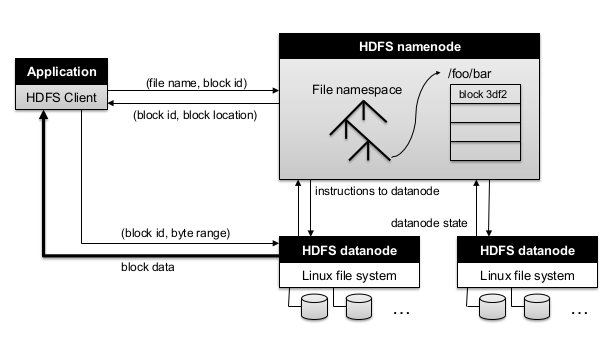
\includegraphics[height=3in]{LaTeX/Chapters/Figures/HDFS.png}
    
  \caption{Arquitetura de HDFS}
  \label{fig:figura-completa}
\end{figure}

\subsection{Coordenação}

\subsubsection{Yarn}
O Yarn \cite{yarn} é um projeto \textit{open-source} desenvolvido pela Apache Software Foundation. A ideia fundamental da tecnologia Yarn é baseada em dois conceitos chave: controlar recursos no \textit{cluster}; e escalonar as tarefas a executar nos diferentes nós do \textit{cluster}.

Existem dois componentes principais, o \textit{Resource Manager} (RM) e o \textit{Node Manager}, que formam a \textit{framework} de computação de dados.
Para controlar todos os recursos o \textit{Resource Manager} desempenha um papel crucial, e só existe uma instância dele pelo \textit{cluster}. Este é a autoridade máxima no que toca a alocar recursos entre todas as aplicações no sistema. O \textit{Node Manager} é responsável por monitorizar os recursos em uso dos \textit{containers}. Os \textit{containers} são os componentes que são alocados pelo \textit{Resource Manager}. Estes são um conjunto de recursos (RAM, numero de CPUs, Network usage, entre outros) que têm como finalidade executar tarefas, como por exemplo, executar uma tarefa de \textit{reduce} ou \textit{map}.

No que toca a escalonar os diferentes tipos de tarefas a executar, o componente \textit{Application Master} (AM) é o responsável. Por norma existe uma instância de AM para cada aplicação existente no sistema. A sua função é negociar com o \textit{Resource Manager} por recursos para a execução de determinada tarefa, e também trabalhar com o \textit{Node Manager} que executa e monitoriza as diferentes tarefas.

\begin{figure}[htbp]
	\centering
	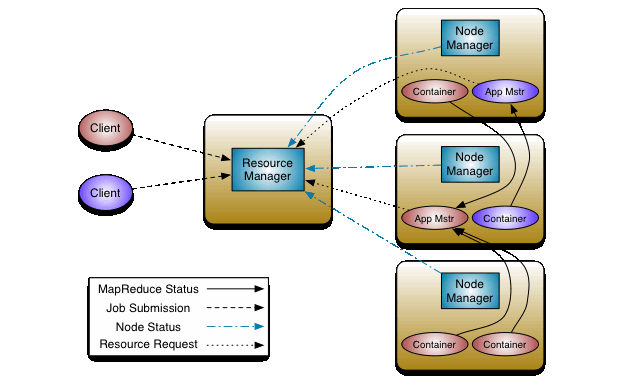
\includegraphics[height=3in]{LaTeX/Chapters/Figures/yarn.png}
    
  \caption{Arquitetura de YARN \cite{yarn}}
  \label{fig:yarn-architeture}
\end{figure}

\subsection{Computação \textit{Cloud}}
O conceito de computação \textit{cloud} trouxe muitas vantagens no que toca ao desenvolvimento de máquinas configuradas em \textit{cluster}, que podem facilmente ser requisitadas a pedido e à medida das necessidades, fazendo com que a carga de processamento possa ser distribuída de uma maneira equilibrada. Um provedor de serviços \textit{cloud} pode oferecer 3 tipos de serviços (todos por via da Internet) ~\cite{lin2010data}:
\begin{description}
    \item[IaaS]: \textit{Infrastructure as a service}, tem como objetivo fornecer aos utilizadores/organizações instâncias de máquinas virtuais, entre outros recursos físicos. Contudo este é um nível que costuma ser muito baixo para grande parte dos utilizadores. Este tipo de serviço oferece uma abstração sobre o hardware, pois muitas das organizações podem não ter o capital ou as competências para construir um centro de dados (\textit{datacenter}).
    
    \item[PaaS]: \textit{Platform as a service}, oferece tanto hardware como software. Estas plataformas são um conjunto bem definido de serviços no qual, permitem aos utilizadores/organizações desenvolver uma aplicação "por cima" \thinspace deste serviço. Um dos exemplos da utilização deste tipo de serviços é a \textit{Google App Engine}, que fornece armazenamento de \textit{backend} e uma API para desenvolver aplicações web altamente 
    escaláveis. Com este serviço os utilizadores/organizações ficam livres de instalar, tanto hardware como software, para desenvolver uma aplicação.
    
    \item[SaaS]: \textit{Software as a service} que está no nível mais alto de abstração, faz \textit{host} de aplicações e deixa-as disponíveis aos seus utilizadores. Um exemplo deste serviço é a empresa Salesforce, que é líder na gestão de relacionamento com o cliente (\textit{Customer Relationship Management, CRM}). Este serviço remove a necessidade das organizações instalarem e correrem as aplicações nas suas próprias máquinas ou centros de dados.
    
\end{description}
Estes serviços oferecem vantagens no desenvolvimento e gestão das infraestruturas (máquinas e restantes recursos) e sua oferta aos utilizadores/organizações. Também procuram facilitar ao utilizador/programador no desenvolvimento de soluções de software que usam essas infraestruturas e serviços \textit{\textit{cloud}}. Uma das vantagens mais relevantes é o facto de se poder alugar recursos computacionais de que outro modo lhes seria impossível adquirir, como por exemplo, \textit{clusters} e armazenamento. Consequentemente, o custo do processamento destes dados só vai ser gasto no momento em que os dados estiverem prontos para serem processados. Ou seja, dá a vantagem ao utilizador de pagar apenas o que usa. Devemos estar conscientes de que, embora o montante global de dados nestes casos realmente excede os limites dos atuais computadores físicos, a frequência tanto da obtenção como do processamento de dados pode ser variável, enfatizando assim o quão útil a computação \textit{\textit{cloud}} é.

As aplicações \textit{web} vistas hoje em dia podem ser chamadas também "aplicações \textit{\textit{cloud}}". De facto, os utilizadores ao acederem a sites web com o seu \textit{browser}, sem saberem, podem estar a usar aplicações que estão a coligir informação sobre a sua utilização e comportamento dos utilizadores. Muitas destas aplicações são suportadas por servidores (possivelmente em \textit{cloud}) com a interface via \textit{browser}. Como por exemplo, serviços de redes sociais como Facebook, sites de partilha de vídeo como Youtube, sites baseados em serviços de email como Gmail, ou aplicações como o Google Docs. Neste contexto o conceito de computação \textit{\textit{cloud}} é um modelo que permite de forma ubíqua, aceder a uma rede com uma \textit{pool} partilhada de recursos computacionais configuráveis (p. e. servidores, armazenamento, aplicações, e serviços) que podem ser rapidamente provisionados e lançados, não requerendo muito esforço em geri-la ~\cite{mell2011nist}. Claro que a vasta quantidade de dados gerada pelos utilizadores cria grandes problemas para processar esses dados em tempo útil.

Com o objetivo de colmatar esta problemática, a primeira \textit{framework} de sucesso em ambiente \textit{\textit{cloud}} que permitiu processar grande quantidade de dados em larga escala foi o \textit{MapReduce}~\cite{dean2008mapreduce}. Esta \textit{framework} pode ser utilizada em serviços de email, para analisar mensagens e o comportamento do utilizador com o objetivo de otimizar a seleção de publicidades adequadas. Ou para analisar grafos enormes que representam as amizades de um utilizador numa rede social (p. e. Facebook), para lhe sugerir novas amizades. Estes são os grandes problemas de dados que o \textit{\textit{MapReduce}} tem atacado~\cite{lin2010data}.

\subsubsection{\textit{\textit{MapReduce}}}
\label{mapreduce_framework}
A abordagem mais eficaz para atacar a problemática de volumes grandes de dados é dividir e conquistar (\textit{divide-and-conquer}), um conceito fundamental à ciência da computação. A ideia base é particionar um grande problema em pequenos sub-problemas. Sendo estes sub-problemas independentes, podem ser processados em paralelo por diferentes trabalhadores (\textit{threads} de um processador, muitos processadores numa máquina, ou muitas máquinas em \textit{cluster}). Resultados intermédios dos vários trabalhadores (máquinas) são combinados, resultando no \textit{output} final~\cite{lin2010data}.

Os princípios por detrás de algoritmos \textit{divide-and-conquer} aplicam-se a um grande leque de problemas em diferentes ramos. Contudo os detalhes das suas implementações são variados e complexos. Aqui estão algumas das questões que devem ser respondidas para desenvolver uma aplicação paralela:
\begin{itemize}
    \item Como partir o problema grande em pequenos sub-problemas?
    \item Como espalhar as tarefas por trabalhadores que estão distribuídos num grande número de máquinas?
    \item Como garantir que os trabalhadores recebem os dados de que precisam?
    \item Como coordenar a sincronização entre os diferentes trabalhadores?
    \item Como partilhamos resultados de um trabalhador que são precisos para outro?
    \item Como conseguimos realizar todas as questões acima face a erros de \textit{software} e falhas no \textit{hardware}?
\end{itemize}
Na programação paralela tradicional o \textit{developer} pode ter de responder e implementar uma solução, na maior parte dos casos a todas as questões acima. Se se programa numa infraestrutura de memória partilhada é necessário coordenar explicitamente os acessos às estruturas de dados partilhada, pelo uso de primitivas de sincronização tais como, \textit{mutexes}, coordenar a sincronização entre as diferentes máquinas, e ainda manter-se atento a possíveis problemas como \textit{deadlocks}. Um sistema como o OpenMP , providencia uma API com abstrações lógicas que escondem os detalhes de sincronização de sistemas e primitivas de comunicação. Contudo, mesmo com estas extensões o programador tem de continuar a preocupar-se em manter disponível os diversos recursos de que cada trabalhador precisa. Além disso, estas \textit{frameworks} são maioritariamente desenhadas para problemas de processamento intensivo e têm um suporte fraco para lidar com quantidades significativas de dados~\cite{lin2010data}. Ficando tal a cargo do programador.

Uma das grandes vantagens que o \textit{MapReduce} tem é o facto de disponibilizar uma abstração de mais alto nível em relação à \textit{framework} de cima. Escondendo muitos detalhes de diferentes níveis do sistema. Isto permite que o \textit{developer} se foque mais no que é que os processamentos precisam para ser executados, em vez de se preocupar como é que essas computações são realmente realizadas ou de como é que os processos obtêm os dados que requerem. Tal como o OpenMP, o \textit{MapReduce} concede os meios de computação paralela e sua distribuição sem sobrecarregar o programador. Organizar e gerir grandes quantidades de computação é só uma parte do desafio. Processar largas quantias de dados requer juntar grandes \textit{datasets}\footnote{Coleção de dados.} a código para ocorrer a computação. A \textit{framework} \textit{MapReduce} resolve este problema de maneira a fornecer um modelo de programação simples ao programador, tratando de forma transparente os detalhes da execução paralela numa maneira escalável, robusta, e eficiente. Por razões de eficiência, em vez de mover grandes montantes de dados, se possível, mover o código pelos nós que possuem os dados. Esta operação consiste em espalhar os dados em discos locais nos nós do \textit{cluster} e correr os processos nos nós que possuem os dados. A tarefa de gerir o armazenamento nos processos, normalmente é tratada por um sistema de ficheiros distribuído que assenta por baixo do \textit{MapReduce}~\cite{lin2010data}.

\textit{MapReduce} é um modelo de programação que tem as suas raízes em programação funcional. Uma das vantagens de linguagens funcionais é que existe o conceito de hierarquia de funções, ou funções que aceitam outras funções como argumento. Para além disto, também existe a diferença de que neste modelo baseamos o programa na avaliação de funções sem necessidade de estado global partilhado entre diferentes contextos de avaliação. Todo o estado é pesado/recebido como parametros da função ou resultados da mesma. Como consequência, não existem problemas de concorrência ou operações explícitas que o programador tenha de usar para a partilha de dados entre diferentes \textit{threads}.

Esta \textit{framework} possui duas fases: a fase do \textit{map} que corresponde à operação \textit{map}\footnote{Dada uma lista, a operação map recebe como unico argumento uma função \textit{f} que aplica a todos os elementos da lista.} em programação funcional; E a fase de \textit{reduce} que corresponde à operação \textit{fold}\footnote{Dada uma lista, a operação fold recebe como argumetos uma função \textit{g} (que tem dois argumentos) e um valor inicial: g é primeiro aplicado ao valor inicial e no primeiro elemento da lista, depois o resultado é guardado em variáveis intermédias.} em programação funcional. Cada computação recebe uma coleção de pares \textit{key/value}, e produz como \textit{output} pares de \textit{key/value}. O utilizador da biblioteca \textit{MapReduce} expressa esta computação com duas funções: \textit{Map} e \textit{Reduce} ~\cite{lin2010data}.

\textit{Map}, escrita pelo utilizador, recebe um par como \textit{input} e produz uma coleção(\textit{set}) de pares intermédios. Esta biblioteca trata de agrupar todos os valores intermédios associados a uma chave X intermédia, e envia-os para a função \textit{Reduce}.

A função \textit{Reduce}, igualmente escrita pelo utilizador, aceita a chave intermédia e uma coleção de valores associados a essa chave. Junta todos esses valores para formar um \textit{set} pequeno de valores. Estes valores intermédios são fornecidos ao utilizador da função reduce por via de um iterador. Isto permite que possamos trabalhar com grandes listas de valores que são demasiado grandes para serem suportadas pela memória~\cite{lin2010data}.

E como é que este modelo pode ser vantajoso para atacar este tipo de problemas? Como exemplo, podemos considerar o exemplo de contar o número de ocorrências de cada palavra em grandes coleções de documentos. Um exemplo de pseudo-código, retirado de ~\cite{dean2008mapreduce}:
\begin{lstlisting}
map(String key, String value):
 // key: document name
 // value: document contents
 for each word w in value:
  EmitIntermediate(w, "1");

reduce(String key, Iterator values):
 // key: a word
 // values: a list of counts
 int result = 0;
 for each v in values:
  result += ParseInt(v);
 Emit(AsString(result));
\end{lstlisting}

A função \textit{map} emite cada palavra com um contador de ocorrências associado (neste exemplo é só '1'). Já o \textit{reduce} soma todos os contadores associados a uma palavra em particular~\cite{lin2010data}.

Esta implementação foca-se apenas no processamento de dados, deixando de fora um grande desafio, a distribuição de dados, que as \textit{frameworks} paralelas oferecem implicitamente, como é o caso da implementação Google de \textit{MapReduce}, ou do sistema \textit{Hadoop} que é similar ao da Google. Recentemente começaram a aparecer outras implementações com modelos de programação mais flexíveis, como \textit{Spark}. Para a temática desta tese foram escolhidas como objeto de estudo, as implementações \textit{Hadoop} e \textit{Spark}.

\subsubsection{\textit{Hadoop}}
\label{hadoop_framework}
O \textit{Hadoop} é um projeto de \textit{open-source} desenvolvido pela Apache Software Foundation. É uma plataforma de computação distribuída, que oferece escalabilidade, confiabilidade e tolerâncias a falhas. Esta implementação, permite processar grandes quantias de dados através de \textit{clusters} de computadores usando o modelo de programação Map Reduce. Em vez de se confiar no hardware para proporcionar maior disponibilidade, a própria \textit{framework} foi concebida para detetar e tratar falhas na camada da aplicação, de modo a fornecer um serviço com alta disponibilidade. Para além da biblioteca base escrita em Java (Hadoop Common), tem também a biblioteca HDFS---\textit{Hadoop Distributed File System}--- e MapReduce~\cite{lin2010data}.

A biblioteca \textit{MapReduce} é análoga ao que foi explicado em cima. O fluxo de execução desta biblioteca consiste em (exemplificado na \ref{fig:fluxo_execucao}, retirado de ~\cite{dean2008mapreduce}): Distribuir as tarefas \textit{map} e \textit{reduce} pelo \textit{cluster} (indicado na figura~\ref{fig:fluxo_execucao} como (2)); Segue-se a leitura dos dados distribuídos, isto é, cada nó que tem a responsabilidade de executar a tarefa \textit{map}, vai executá-la sobre os dados que possuí (indicado na figura~\ref{fig:fluxo_execucao} como (3)); A função \textit{map} produz resultados intermédios, resultados estes que vão ser guardados no disco local e ordenados (indicado na figura~\ref{fig:fluxo_execucao} como (4)); de seguida procede-se à execução concorrente dos nós que foram designados para a execução da tarefa \textit{reduce}; estes vão receber uma chave juntamente com um iterador de todos os valores que lhe correspondem e vai agregá-los num só resultado (indicado na figura~\ref{fig:fluxo_execucao} como (5)); A fase final consiste na obtenção dos dados produzidos pelos \textit{reducers} (indicado na figura~\ref{fig:fluxo_execucao} como (6)).

\begin{figure}[htbp]
	\centering
	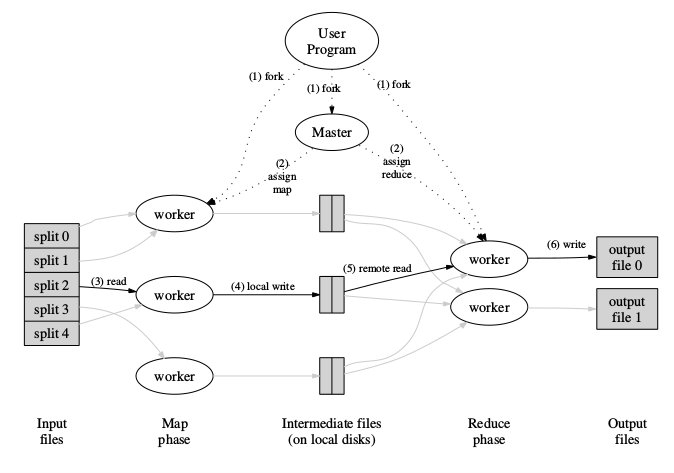
\includegraphics[height=3in]{LaTeX/Chapters/Figures/MapReduceExecutionFlow.jpg}
  \caption{Fluxo de Execução \textit{Hadoop}}
  \label{fig:fluxo_execucao}
\end{figure}


\subsubsection{\textit{Spark}}
\label{estadoARte_spark}
Tanto o \textit{MapReduce}, como as suas variantes que foram criadas ao longo do tempo, têm tido muito sucesso na implementação de aplicações escaláveis e de grandes montantes de dados em \textit{clusters}. No entanto, elas pecam por serem construídas num modelo de fluxo de dados acíclico. Isto é, aplicações que não reutilizam coleções de dados para múltiplas operações em paralelo. A \textit{framework Spark} propõe suportar este tipo de aplicações, mantendo ainda assim a escalabilidade e tolerância a falhas do \textit{MapReduce}. Para atingir esta finalidade uma das abstrações oferecidas é chamada \textit{resilient distributed datasets} (RDDs). RDD é uma coleção de objetos particionados, só de leitura, por várias máquinas~\cite{zaharia2010spark}. 

A abordagem para as aplicações que reutilizam coleções de dados, incluí também dois casos cujos utilizadores de \textit{Hadoop} revelaram o \textit{MapReduce} falhar:
\begin{itemize}
    \item Execuções iterativas: Muitos dos algoritmos de aprendizagem automática aplicam repetidas vezes a mesma função à mesma coleção de dados para otimizar parâmetros. Sendo cada iteração expressada num processo \textit{MapReduce}, cada processo vai ter de carregar dados do disco, fazendo com que haja um declínio na performance.
    \item Análise interativa: O ambiente \textit{Hadoop} é regularmente usado para pesquisas \textit{ad-hoc} em grandes coleções de dados, por via SQL, com interfaces como \textit{Pig} e \textit{Hive}. O ideal seria o utilizador ser capaz de carregar uma porção da coleção de dados do seu interesse para memória, através de várias máquinas, e pesquisar sobre essa coleção as vezes que bem entender. No entanto, no \textit{Hadoop}, cada pesquisa ocorre com alguma latência porque executa como um processo \textit{MapReduce} e lê dados do disco.
\end{itemize}

Para usar \textit{Spark}, os utilizadores escrevem um programa principal (\textit{driver program}) que implementa o controlo de alto nível do fluxo da aplicação, e lança as várias operações em paralelo. Este ambiente fornece duas abstrações principais: \textit{resilient distributed datasets} e operações paralelas. 
Os elementos de um \textit{resilient distributed datasets} (RDD) não necessitam de existir em armazenamento persistente, porque um identificador de RDD contém informação suficiente para calcular o RDD a partir de dados em armazenamento confiável. Isto quer dizer que o RDD pode sempre ser reconstruído se um nó que o continha falhou.
Existem dois tipos de operações paralelas que podem executar sobre os RDDs:
\begin{itemize}
    \item \textit{transformações}, que vão criar um novo \textit{dataset} (RDD) de um já existente. Exemplo: \textit{map(func), mapPartitions(func), reduceByKey(func, [numTasks])};
    \item \textit{ações}, que retornam os valores ao \textit{driver program} depois da computação ser efectuada no RDD. Exemplo: \textit{reduce(func), collect(), saveAsTextFile()}
\end{itemize}

Este ambiente não suporta uma operação \textit{reduce} análoga à \textit{framework MapReduce}, pois todos os resultados são recolhidos no programa principal. Apesar de existir pequenas reduções locais nos nós~\cite{zaharia2010spark}. Este modelo pode ser vantajoso em vários aspetos.

Considerando um exemplo que conta o número de ocorrências de cada palavra em grandes coleções de documentos (retirado de ~\cite{apacheSparKExample}):
\begin{lstlisting}
val textFile = sc.textFile("hdfs://...")
val counts = textFile.flatMap(line => line.split(" "))
                 .map(word => (word, 1))
                 .reduceByKey(_ + _)
counts.saveAsTextFile("hdfs://...")
\end{lstlisting}

A função \textit{mapToPair} vai criar um par (String, Integer) para cada palavra que lê, enquanto que a função \textit{reduceByKey} faz uma redução local, somando todos os valores de chaves iguais.

\subsubsection{\textit{Spark vs \textit{Hadoop}}}
Estas duas plataformas têm ambas o propósito de tratar problemas de Big Data, no entanto servem propósitos diferentes. O \textit{Hadoop} é essencialmente uma infraestrutura de dados distribuída. Distribuí quantidade enormes de dados por múltiplos nós num \textit{cluster}. Mantêm também um índice para todos os blocos de dados juntamente com o sítio onde eles estão alojados, permitindo assim a análise e processamento mais eficientes. Enquanto que o \textit{Spark}, não oferece qualquer tipo de infraestrutura de dados distribuída, focando-se apenas uma plataforma de processamento de dados. 

No geral, podemos constatar que o \textit{Spark} é mais rápido que o \textit{MapReduce} por causa da maneira como processa os dados. O fluxo de trabalhos do \textit{MapReduce} consiste em: ler dados do \textit{cluster}, executar operação, escrever resultados para disco, ler dados actualizados do \textit{cluster}, executar operação, sempre neste ciclo. Por outro lado, o \textit{Spark} executa todas as operações de análise sobre os dados em memória e em tempo real. Traduz-se em: Ler dados de um \textit{cluster}, executar todas as operações de analise, escrever resultados no \textit{cluster}. Isto permite que este ambiente seja mais rápido do que o \textit{MapReduce} em processamento \textit{batch}\footnote{Processamento batch é a analise de uma coleção de dados fixa.} e muito mais rápido para analisar dados em memória. 

Considerando algumas das divergências entre estas duas plataformas, ainda não foi formada um opinião em relação ao ambiente a utilizar. No entanto, irão ser feitos mais testes para concluir qual será o ambiente ideal a integrar o protótipo a desenvolver nesta tese.

\section{Machine Learning}

\subsection{Word2Vec}
O Word2Vec é um projecto que foi criado por uma equipa de investigação liderada por Tomás Mikolov na Google. Esta técnica é feita com base em redes neuronais, redes que, por isso mesmo, têm de ser previamente treinadas. Tipicamente esta abordagem toma como \textit{input} corpora linguísticos de médias/grandes dimensões e produz como resultado vetores com muitas dimensões, em que cada palavra do corpus é representada por um vetor nesse espaço vetorial\cite{word2vec}. 

Tendo isto em conta, o Word2vec consegue posicionar palavras num espaço vetorial atendendo ao contexto onde elas surgem no texto. No entanto, não contempla o conceito de Expressão Relevante e a sua potencialidade na captura do valor semântico do grupo de palavras relevantes, semântica essa que não é capturada com a simples agregação semântica das palavras individuais que constituem a expressão relevante. Por exemplo a expressão "raining cats and dogs", não significa que chovem cães e gatos, mas sim que está a chover imenso. 

O nosso protótipo pretende construir descritores de documentos, baseados em \textit{keywords} automaticamente extraídas dos documentos. As \textit{keywords} correspondem às melhores Expressões Relevantes. Nesta medida, o word2vec não oferece potencialidade para ser uma solução para o problema, pois a noção de expressão relevante não é contemplada nessa técnica. Quanto às \textit{keywords} implícitas, o word2vec poderia ser uma solução, no sentido em que consegue determinar a "distância semântica" entre palavras, mas ainda assim, não determina essa distância aplicada a Expressões Relevantes (tipicamente, conjuntos de 2 ou mais keywords, n-grams).

Quanto ao paralelismo, julgo não haver à partida nenhuma impossibilidade de o cálculo relativo do posicionamento das palavras pelo word2vec, ser feito em paralelo, depois de construída a rede neuronal. No entanto, põe-se sempre a questão de não satisfazer a condição das expressões relevantes.